\documentclass[titlepage,a4paper]{article}

\usepackage{a4wide}
\usepackage[colorlinks=true,linkcolor=black,urlcolor=blue,bookmarksopen=true]{hyperref}
\usepackage{bookmark}
\usepackage{fancyhdr}
\usepackage[spanish]{babel}
\usepackage[utf8]{inputenc}
\usepackage[T1]{fontenc}
\usepackage{graphicx}
\usepackage{float}
\usepackage{listings}

% +--- VARIABLES ---+
\newcommand{\FirstName}{Carlos E.}
\newcommand{\LastName}{Castillo}
\newcommand{\StudentID}{108535}
\newcommand{\StudentEmail}{ccastillo@fi.uba.ar}
% \newcommand{\ProjectName}{Trabajo Práctico n — NombreTP}
\newcommand{\ProjectName}{TDA 1 — Lista, Pila y Cola}

\pagestyle{fancy}
\fancyhf{}
\fancyhead[L]{TP - \FirstName \LastName}
\fancyhead[R]{Algoritmos y Programación II - FIUBA}
\renewcommand{\headrulewidth}{0.4pt}
\fancyfoot[C]{\thepage}
\renewcommand{\footrulewidth}{0.4pt}

\begin{document}
\begin{titlepage}
	\hfill
\includegraphics[width=6cm]{logofiuba.jpg}
    \centering
    \vfill
    \Huge \textbf{\ProjectName}
    \vskip2cm
    \Large [7541/9515] Algoritmos y Programación II\\
    Segundo cuatrimestre de 2021 
    \vfill
    \begin{tabular}{ | l | l | }
      \hline
      Alumno: & \LastName, \FirstName \\ \hline
      Número de padrón: & \StudentID \\ \hline
      Email: & \StudentEmail \\ \hline
  	\end{tabular}
    \vfill
    \vfill
\end{titlepage}

\tableofcontents
\newpage

\section{Introducción}\label{sec:intro}

Muchos lenguajes de programación permiten al usuario extender los tipos de datos nativos del lenguaje con para facilitar la implementación de características y funcionalidades más complejas. 
De esta forma, el programador tiene la capacidad de combinar diferentes primitivas del lenguaje y así generar nuevos tipos compuestos para crear interfaces abstractas que faciliten el manejo y organización de la información mediante diferentes estructuras de datos.

El objetivo de este trabajo práctico es implementar una de las estructuras de datos más populares, la lista enlazada, así como dos de sus derivados, pila y cola.

\section{Teoría}\label{sec:teoria}

\subsection{TDA Lista}

Una lista es una colección lineal de datos cualquiera, en la que los elementos son colocados el uno al lado del otro. Una lista permite al usuario insertar nuevos elementos, ya sea al final de la lista o en una posición específica, borrar elementos en cualquier posición, buscar algún elemento en particular o revisar si la lista esta vacía. Además el usuario puede crear o destruir nuevas listas. A priori la funcionalidad de este tipo de dato se asemeja mucho a la funcionalidad de un arreglo.

Existen muchas implementaciones de lista como listas implementadas con vectores estáticos, listas implementadas con vectores dinámicos o listas circulares, pero en particular, una de las más interesantes es la implementación de lista enlazada compuesta por nodos, donde un nodo es otro tipo de dato abstracto que además de almacenar el elemento en cuestión, puede conocer al nodo que le sucede o que le antecede.

\subsubsection{Lista Enlazada}

La implementación de lista basada en nodos enlazados permite el almacenamiento no secuencial de los datos en memoria, lo que significa que cada uno de los elementos individuales puede ser almacenado en cualquier otra parte de la memoria. Para mantener el la estructura lineal y continua de la lista establecida por el usuario, se utiliza alguna de las referencias que cada nodo tiene con respecto a su antecesor o sucesor, así se puede recorrer la lista de nodo en nodo ordenadamente, avanzando al nodo siguiente en cada caso. En algunos tipos de lista enlazada, conocidas como listas doblemente enlazadas, cada nodo puede tener al mismo tiempo una referencia a su antecesor y sucesor, lo que permite tanto ''avanzar'' como ''retroceder'' en cualquier punto de la lista.

Esta forma de organizar los datos en memoria facilita muchas de las operaciones de la lista, principalmente la inserción y eliminación de elementos, ya que, como los elementos no están almacenados en bloques de memoria continuos, cuando se agrega o se quita un elemento en particular no es necesario que se le reasigne memoria a la lista ni que se tengan que reorganizar todos los demás elementos de la misma.

\subsection{TDA Pila y Cola}

De la estructura de datos lista se pueden derivar otras dos estructuras similares, conocidas como pila y cola, las cuales también pueden ser construidas a partir de nodos. Además de esta versión, existen otras variantes de estas estructuras, que pueden o no implementarse a partir de una lista enlazada, como lo son la pila con vector estático o dinámico, cola con vector estático, cola con vector dinámico y cola circular, creada con la intención de reutilizar un vector estático en una cola.

Las operaciones de pila y cola divergen levemente de las operaciones del tipo lista, aunque para una implementación basada en nodos, estas operaciones pueden ser consideradas casos particulares de las operaciones estándar de una lista enlazada.

La estructura de datos pila consiste en una colección de elementos organizados de manera lineal en las que solo se tiene acceso al elemento que se encuentra en el tope de la pila, es decir, el último elemento agregado. De esta forma, al agregar un elemento a la pila, solamente se puede agregar sobre el tope actual de la misma. De igual manera, solamente se puede quitar el último elemento de la pila. Esto implica que para quitar un elemento en medio de la pila, primero se tienen que quitar todos los elementos que fueron agregados después de ese elemento, o los elementos que están encima. Este método para agregar y quitar elementos es conocido como \textbf{LIFO} (del inglés ''Last In First Out''), que se traduce como ''ultimo en entrar, primero en salir''. Visto como caso particular de una lista enlazada, el agregar (o ''apilar'') un elemento en una pila equivale a agregar un elemento únicamente al final de la lista, y el quitar (o ''desapilar'') elemento es equivalente a quitar solamente el último elemento de la lista.

Por otra parte, el tipo de dato cola consiste también en una colección secuencial de datos en el que solo se tiene permitido agregar (o ''encolar'') elementos al final de la cola, sin embargo, contrario a lo sucede en una pila, en una cola solo se tiene acceso al elemento que está al frente de la cola, es decir, al primer elemento insertado. De esta forma, si se desea sacar un (o ''desencolar'') elemento se tienen que remover el primer elemento de la cola. Este método para agregar y quitar elementos es conocido como \textbf{FIFO} (del inglés ''First In First Out''), que se traduce como ''primero en entrar, primero en salir''.


\section{Detalles de implementación}\label{sec:implementacion}

La implementación de estas tres estructuras de datos fue escrita en el lenguaje de programación C, siguiendo la especificación del lenguaje detallada en el estándar C99. Los archivos principales se encuentran dentro del directorio \textbf{src} ubicada en la raíz del repositorio. 

Además se incluye un archivo \textbf{pruebas.c} en el que se encuentran diferentes pruebas automatizadas para detectar errores en la ejecución del programa o en la asignación, manejo y liberación de memoria dinámica. Para esto se utiliza \textbf{gcc} como compilador y \textbf{valgrind} como herramienta de análisis de memoria.

La estructura de lista propuesta para esta implementación es la siguiente:

\begin{lstlisting}
  struct lista {
    nodo_t* nodo_inicio;
    nodo_t* nodo_fin;
    size_t cantidad;
  };
\end{lstlisting}

Los TDAs pila y cola se derivan de esta misma misma estructura. Para esto se utiliza casteos de punteros de los tipos \lstinline{pila_t} y \lstinline{cola_t} al tipo \lstinline{lista_t}, para que de esta manera también se puedan reutilizar muchas de las funciones que implementan la funcionalidad básica de la lista con las estructuras de pila y cola.

\subsection{Inserción de elementos}
Se proveen dos funciones para insertar elementos. La primera de estas, \lstinline{lista_insertar} se encarga de insertar un elemento al final de la lista y \lstinline{lista_insertar_en_posicion} se encarga de insertar un elemento en la posición especificada por el usuario. Para esta última función, en el caso de que el usuario quisiera agregar un elemento en una posición que no existe en la lista, el elemento se agregará al final de la misma.

Para insertar un elemento en una lista compuesta por nodos enlazados, es necesario cambiar las referencias de los nodos que anteceden y suceden a la posición en la que se quiere ubicar el nuevo elemento. Esta operación tiene varios casos particulares, y para cada uno de estos casos existe una solución específica:

\begin{itemize}
  \item \textbf{Insertar en una lista vacía:} En este caso la implementación de lista cuenta con dos referencias al primer y último nodo de la lista. Al insertar el primer elemento de una lista vacía, se deben apuntar ambos nodos al mismo elemento.
  \item \textbf{Insertar al inicio de la lista:} Para insertar en esta posición, nuevamente se saca provecho de la existencia de la referencia a un nodo inicial de la lista. Al agregar un elemento en la primera posición primero se establece que el nodo siguiente al nodo que va a ser insertado, es decir, el segundo nodo, va a ser el nodo que actualmente está al inicio de la lista. Luego se cambia referencia la referencia al primer nodo de la lista de tal modo que el nodo que contiene al elemento agregado sea el nuevo primer nodo de la lista. 
  \item \textbf{Insertar al final de la lista:} La operación de insertar en esta posición puede ser vista como la inversa de la operación anterior. Esta vez se utiliza la referencia al elemento que actualmente está al final de la lista, se establece que el elemento siguiente a este último va a ser el nuevo nodo insertado, y finalmente se cambiar la referencia del último nodo de la lista hacia el nuevo nodo.
  \item \textbf{Insertar en cualquier posicion:} Para insertar en cualquier posición de la lista se debe hacer un cambio de referencias similar al de los casos anteriores. Primero se tiene que ubicar el nodo que actualmente se encuentra en la posición anterior a la deseada. Se copia la referencia de este nodo a su nodo siguiente (el nodo que está en la posición deseada) de tal forma que el nuevo nodo a insertar apunte hacia este nodo, y finalmente se hace que el nodo que anterior a la posición deseada tome como nuevo siguiente el nodo que se está insertando.
\end{itemize}

Por último se aumenta la cantidad de elementos en la lista y se retorna el puntero a la lista nuevamente.

Cada destacar que la función \lstinline{lista_insertar} fue implementada de tal manera que esta fuera solamente una manera auxiliar de llamar a la función \lstinline{lista_insertar_en_posicion} especificando la última posición de la lista.

Para la operación de apilado en una pila, se utiliza la misma funcionalidad de inserción que para la lista pero especificando el tope de la pila (posición final) como la única posición de insertado. Por otra parte, para la operación de encolado en una cola, se utiliza esta misma función, nuevamente especificando la posición final de la cola como única posición de insertado posible.


\subsection{Eliminación de elementos}

La operación de quitar elementos de la lista tiene una implementación bastante similar a la operación de insertado. También se proveen dos funciones para quitar elementos tanto del final de la lista con la función \lstinline{lista_quitar}, así como también para quitar un elemento de cualquier posición con la función \lstinline{lista_quitar_en_posicion}, la primera de estas funciones siendo un auxiliar de la segunda, en el que se especifica que la posición de eliminado es la última en el caso de la lista.

Al igual que con la inserción de elementos, existen varios casos particulares de eliminación:

\begin{itemize}
  \item \textbf{Quitar del inicio de la lista:} En esta operación se guarda una referencia al nodo a quitar (el primer nodo de la lista) y posteriormente se apunta la referencia de la lista hacia el nuevo primer nodo (que anteriormente era el segundo). Finalmente se almacena el valor que contiene el nodo para retornarlo y se libera la estructura nodo que se removió de la lista.
  \item \textbf{Quitar del final de la lista:} Para quitar un elemento del final de la lista simplemente se guarda una referencia a ese nodo, luego se apunta la referencia de la lista al nodo final hacia el nodo anterior (que anteriormente era el penúltimo), y finalmente se almacena el valor que contiene el nodo para retornarlo y se libera la estructura nodo que se removió de la lista. Al tener una referencia al final de la lista, no se tiene la necesidad de recorrer toda la lista para encontrar el final, así que el tiempo de inserción en el final de la lista es constante si no se requiere de una operación adicional.
  \item \textbf{Quitar de cualquier posición:} Para quitar un elemento de cualquier posición se realiza una operación similar al insertado en cualquier posición, en la que primero guarda una referencia al nodo que se va a eliminar. Luego se localiza el nodo anterior a la posición que se desea quitar en este caso, se cambia la referencia al siguiente nodo para este nodo, y pasa ser el nodo siguiente al que se va a remover. Finalmente se guarda el valor del nodo a quitar para que pueda ser devuelto y se libera la estructura nodo de la memoria.
\end{itemize}

Para las implementaciones de los TDAs pila y cola también se trabaja con las funciones de lista para la operación de remover elementos. En el caso del desapilado en la pila se especifica la única opción de desapilado posible como la posición del tope de la pila (misma posición del último elemento apilado), y para el caso del tipo de dato cola, se especifica la posición de desencolado como la posición del primer nodo de la cola, es decir siempre el que siempre está al frente.

\subsection{Otras operaciones}

Además de las operaciones de insertar y quitar se proveen una serie de getters para cada tipo de dato. En el caso de la lista, el usuario puede acceder al primer y último elemento de la misma sin necesidad de remover el elemento, así como también puede acceder a cualquier elemento en medio de la lista. Para acceder al primer y último nodo se utilizan las funciones \lstinline{lista_primero} y \lstinline{lista_ultimo} que toman provecho de las referencias que tiene la lista hacia el nodo inicial y final para realizar esta operación en tiempo constante. Por otra parte, para acceder a cualquier otro elemento se utiliza la función \lstinline{lista_elemento_en_posicion}, la cual si tiene que hacer un recorrido a traves de la lista hasta que encuentra el elemento buscado o \lstinline{NULL} si no se encuentra.

En el caso del tipo de dato pila solo se provee un getter para acceder al elemento del tope, y para el tipo de dato cola, solamente para acceder al elemento del frente.

Para las tres estructuras de datos existen funciones que se encargan de la construcción y destrucción de las mismas, sin destruir la información que tiene almacenada el usuario. Además, las tres estructuras tienen una función retorna la cantidad de elementos que contienen en el momento y otra función que determina si la estructura está vacía o no.


\section{Diagramas}\label{sec:diagramas}

\begin{figure}[H]
\centering
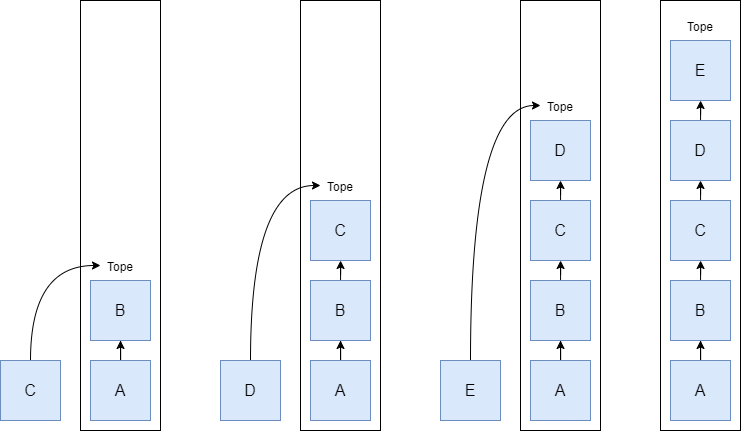
\includegraphics[width=0.8\textwidth]{pila_apilado.png}
\caption{\label{fig:seq01}Apilado en pila.}
\end{figure}


\begin{figure}[H]
\centering
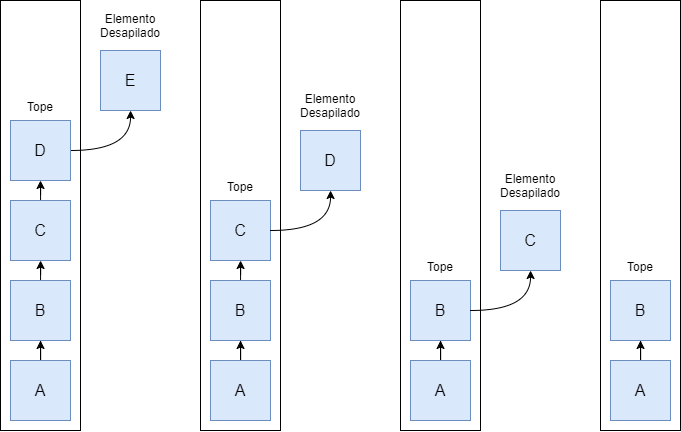
\includegraphics[width=0.8\textwidth]{pila_desapilado.png}
\caption{\label{fig:seq02}Desapilado en pila.}
\end{figure}


\begin{figure}[H]
\centering
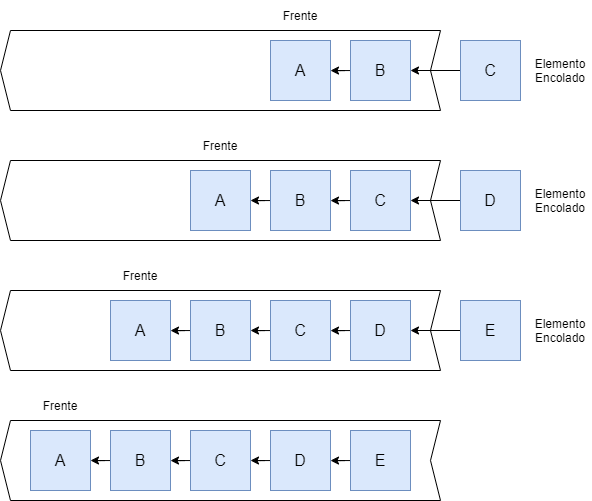
\includegraphics[width=0.8\textwidth]{cola_encolado.png}
\caption{\label{fig:seq03}Encolado en cola.}
\end{figure}


\begin{figure}[H]
\centering
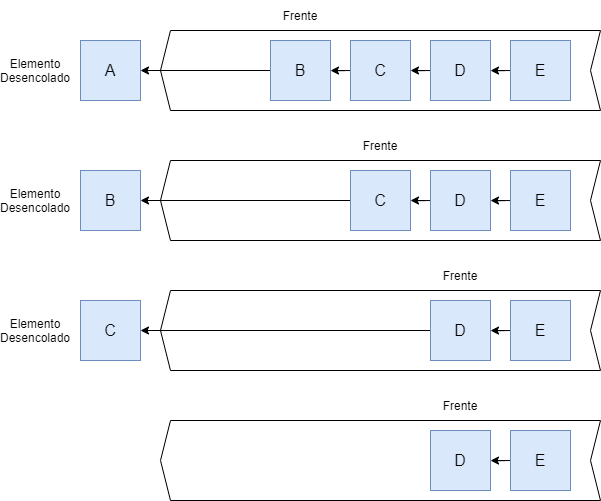
\includegraphics[width=0.8\textwidth]{cola_desencolado.png}
\caption{\label{fig:seq04}Desencolado en cola.}
\end{figure}


\begin{figure}[H]
\centering
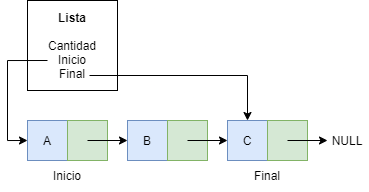
\includegraphics[width=0.8\textwidth]{lista_general.png}
\caption{\label{fig:seq05}Implementación de lista enlazada.}
\end{figure}


\begin{figure}[H]
\centering
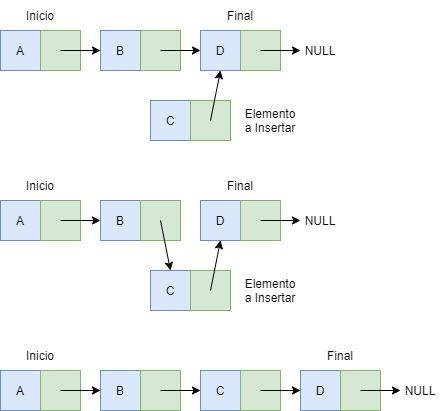
\includegraphics[width=0.8\textwidth]{lista_insercion.png}
\caption{\label{fig:seq06}Insertado en lista.}
\end{figure}


\begin{figure}[H]
\centering
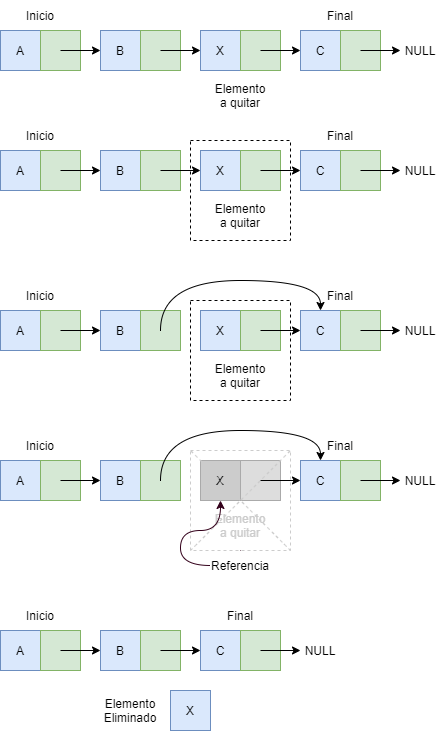
\includegraphics[width=0.8\textwidth]{lista_quitar.png}
\caption{\label{fig:seq07}Eliminación en lista.}
\end{figure}


\end{document}
